\documentclass[a4paper, 11pt]{article} % Font size (can be 10pt, 11pt or 12pt) and paper size (remove a4paper for US letter paper)
\usepackage{helvet}
\renewcommand{\familydefault}{\sfdefault}
\usepackage[protrusion=true,expansion=true]{microtype} % Better typography
\usepackage{graphicx} % Required for including pictures
\usepackage[usenames,dvipsnames]{color} % Coloring code
\usepackage{wrapfig} % Allows in-line images
\usepackage[utf8]{inputenc}
\usepackage{enumerate}
\usepackage{enumitem}
\usepackage{framed, color}
\definecolor{shadecolor}{rgb}{0.690, 0.933, 0.525}

% Imágenes
\usepackage{graphicx}

\usepackage{amsmath}
% para importar svg
%\usepackage[generate=all]{svgfig}

% sudo apt-get install texlive-lang-spanish
\usepackage[spanish]{babel} % English language/hyphenation
\selectlanguage{spanish}
% Hay que pelearse con babel-spanish para el alineamiento del punto decimal
\decimalpoint
\usepackage{dcolumn}
\newcolumntype{d}[1]{D{.}{\esperiod}{#1}}
\makeatletter
\addto\shorthandsspanish{\let\esperiod\es@period@code}
\makeatother

\usepackage{longtable}
\usepackage{tabu}
\usepackage{supertabular}

\usepackage{multicol}
\newsavebox\ltmcbox

% Para algoritmos
\usepackage{algorithm}
\usepackage{algorithmic}
\usepackage{amsthm}

% Para matrices
\usepackage{amsmath}

% Símbolos matemáticos
\usepackage{amssymb}
\usepackage{accents}
\let\oldemptyset\emptyset
\let\emptyset\varnothing

\usepackage[hidelinks]{hyperref}

\usepackage[section]{placeins} % Para gráficas en su sección.
\usepackage[T1]{fontenc} % Required for accented characters
\usepackage{tikz}
\newenvironment{allintypewriter}{\ttfamily}{\par}
\setlength{\parindent}{0pt}
\parskip=8pt
\linespread{1.05} % Change line spacing here, Palatino benefits from a slight increase by default

\makeatletter
\renewcommand\@biblabel[1]{\textbf{#1.}} % Change the square brackets for each bibliography item from '[1]' to '1.'
\renewcommand{\@listI}{\itemsep=0pt} % Reduce the space between items in the itemize and enumerate environments and the bibliography
\newcommand{\imagen}[2]{\begin{center} \includegraphics[width=90mm]{#1} \\#2 \end{center}}
\newcommand{\RFC}[1]{\href{https://www.ietf.org/rfc/rfc#1.txt}{RFC-#1}}

\renewcommand{\maketitle}{ % Customize the title - do not edit title and author name here, see the TITLE block below
\begin{center} % Center align
{\Huge\@title} % Increase the font size of the title
\end{center}

\vspace{20pt} % Some vertical space between the title and author name

\begin{flushright} % Right align
{\large\@author} % Author name
\\\@date % Date

\vspace{40pt} % Some vertical space between the author block and abstract
\end{flushright}
\renewcommand{\baselinestretch}{0.5}

}


\usepackage[a4paper]{geometry}
\geometry{top=2cm, bottom=2cm, left=2.25cm, right=2.25cm}

%----------------------------------------------------------------------------------------
%	TITLE
%----------------------------------------------------------------------------------------

\title{\textbf{Búsquedas en Internet}\\ % Title
\vspace{20 pt}
Ingeniería de sistemas de información} % Subtitle

\author{\textsc{Daniel López García\\
Lothar Soto Palma} % Author
\\{\textit{Universidad de Granada}}} % Institution

\date{\today} % Date

\newcounter{ndef}

\begin{document}
	\maketitle
	\tableofcontents
	\listoffigures
	\newpage

	\section{Introducción}
	Actualmente los motores de búsqueda son necesarios en nuestras vidas, cuando un usuario tiene una necesidad de información se dirige a una fuente de conocimiento para intenter suplirla, debido al reciente crecimiento del número de webs, Internet se ha convertido en una fuente de conocimiento masiva, como consecuencia los motores de búsqueda web se han vuelto muy importantes y la necesidad de obtener una arquitectura para estos sistemas que óptimice la realización de búsquedas es ahora una necesidad. En este documento vamos a analizar cada uno de los elementos de la arquitectura de un motor de búsqueda.

	Pero antes de eso es necesario conocer el entorno en el que trabajan dichos motores de búsuqeda:
	\section{La WWW}
	La WWW o World Wide Web es un sistema de distribución de documentos de hipertexto que están interconectados y son accesibles vía internet. El usuario a través de un navegador web visualiza el contenido proporcionado por la web compuesto por elementos multimedia y texto.

	Pero la web es un entorno con unas características un poco adversas a la hora de poder hacer búsquedas sobre ellas esto es debido a su escala, volatilidad y variabilidad de la calidad de las mismas.

	En la web no hay un diseño general, aparte de incluir información verídica puede incluir información obsoleta y contradicciones, el contenido es generado dinámicamente en el tiempo por lo que es necesario volver a analizar cada web para incluirlas en los resultados de las búsquedas de forma rutinaria y por último tiene un gran crecimiento llegando a duplicarse cada pocos meses.

	\section{Busquedas en internet}
	Un buscador web tiene que tener conocimiento de todas las webs para satisfacer las consultas de los usuarios la manera de hacer esto puede diferir dependiendo del sistema utilizado, el proceso más común es la construcción de un índice invertido donde las palabras de cada página son añadidas al índice que están enlazadas con los documentos en los que se encontró la palabra. El motor de búsqueda unicamente se encarga de escanear el índice para determinar los documentos que contienen las palabras de las que se compone la consulta y estos se añaden al conjunto de resultados.
		
	Para realizar una consulta sobre internet es necesario indexar las páginas de las que se compone para ello es necesaria la paralelización y el uso de miles de máquinas, si tuvieramos 5000 máquinas podriamos indexar un billón de páginas aproximadamente en un día pero Internet es varias magnitudes más grande por lo que se necesita aumentar el número de máquinas y una forma inteligente de elegir que páginas webs indexar y cómo. 
	
	Pero hay otros problemas como el almacenamiento del índice, normalmente este no puede ser alojado en una única máquina asi que la cantidad de datos tiene que ser distribuido entre los discos de cada máquina. Además la distribución de los datos de al almacenamiento también ayuda al rendimiento de la consulta, la tarea de escanear las secciones de las webs y combinar las coincidencias en una etapa posterior.
	 
	\section{Modelo de arquitectura referente de motores de búsqueda}
	\subsection{Elementos del modelo}
	Los motores de búsqueda que operan en internet tienen comunmente una arquitectura centralizada, los elementos que componen esta arquitectura son:
	\begin{figure}[H]
	    \centering
    	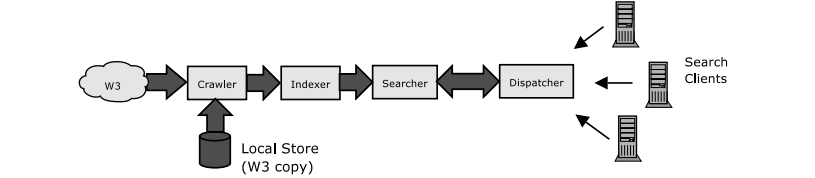
\includegraphics[scale=0.75]{./img/modeloreferente.png}
	    \caption{Modelo de referencia}
	    \label{fig:my_label}
	\end{figure}
		\begin{itemize}
			\item \textbf{Crawler}: Un crawler o una araña es normalmente un módulo que se encarga de la agregación al sistema de los documentos que posteriormente serán indexados para su búsqueda. De forma obvia la obtención de documentos de Internet no es una cuestión sencilla de resolver debido a la naturaleza descentralizada de la web. El funcionamiento básico de un crawler o araña es:
				\begin{verbatim}
					- Partimos de un conjunto semilla de URLs iniciales
					- Establecemos una cola con prioridad en la que se irán incluyen las URLs anteriores
					- Para cada URL de la cola:
					    - Descargamos el contenido de la web
					    - Estraemos los términos de indexación
					    - Incluimos los links de la web en la cola con prioridad
					    - Se vuelve a añadir a la cola la URL analizada
				\end{verbatim}
				Pero este proceso básico no es lo único a tener en cuenta de hecho las arañas suelen necesitar la ayuda de los servidores webs que analizan, con la aportación de datos que permiten entre otras cosas excluir webs del servidor de la araña o moderar el número de peticiones por minuto.

				Existen muchas heurísticas y algoritmos para el crawling y la mayoria de ellos se basan en el análisis de hipertexto en los documentos.
			\item \textbf{Indexer}: El indexador es el módulo que se encarga de a partir de los datos obtenidos con el proceso de crawling construir una estructura de acceso rápido (normalmente una tabla hash) llamada índice. Existen diversos modelos de indexación algunos de ellos son:

				\begin{itemize}
					\item Modelo binario: La interpretación principal de este modelo consiste en en la elaboración de un índice centrandose en la aparición o no de los términos en los documentos.
					\item Modelo Vectorial: Este modelo a diferencia del alterior tiene en cuenta la frecuencia de aparición de un término en los documentos (tf), sin embargo a lo largo del tiempo han surgido modelos que tienen en cuenta la frecuencia inversa de aparición de un término en un documento (idf), y otro modelo que combina las dos ideas anteriorer llamado modelo tf-idf.
					\item Modelo Probabilistico: El modelo probabilistico se centra en la probabilidad de aparición de un término en un documento.
				\end{itemize}
			\item \textbf{Searcher}: El buscador es aquel módulo que normalmente se encarga de el procesamiento de las consultasque se realizan normalmente a través de un entorno web con un navegador, es el encargado de la realización de consultas sobre el índice creado por el indexador anterior.
			\item \textbf{Dispatcher}: Por último el dispatcher es el encargado de la recepción de la consulta realizada desde el buscador y enviarla al buscador que realizará el cotejamiento con el índice para posteriormente obtener una lista ordenada por una puntuación denominada relevancia de URLs que será mostrada a los usuarios a traves del cliente.
		\end{itemize}

		\subsection{Medida de relevancia}
		El grado de relevancia de un documento web es un medida que resulta necesaria definir para que el resto de procedimientos puedan trabajar correctamente, sin embargo la definición de esta medida no es simple puesto que depende normalmente del modelo de indexación que se lleve a cabo. La relevancia de un documento normalmente depende directamente de la consulta que se ha realizado, pero hay algunos casos en elas que se supone que la relevancia puede verse como la suma de dos componentes una que depende de la consulta llamada componente dinámica y otra que no depende llamada componente estática, por supuesto esta no es la única forma de medir la relevancia ya que no hay un método específico, otros ejemplos son:
		\begin{itemize}
			\item Coeficiente de Jaccard en modelos de indexación binarios.
			\item Coseno en modelos de indexación vectorial de tipo tf-idf.
		\end{itemize}
		
	\section{Modelo de arquitectura del motor de búsqueda de Google}
		\subsection{Metodología}
		Partiendo del modelo de arquitectura más general, vamos a ver algunos detalles particulares que incluye Google para optimizar los resultados de las búsquedas.
		\begin{itemize}
			\item Las estructuras de datos usadas están optimizadas para manejar grandes colecciones de datos.
			\item Se hace uso del modelo MapReduce para la creación de los índices.
			\item El crawling se realiza usando una gran cantidad de crawlers de forma distribuida.
			\item Las páginas webs obtenidas mediante el crawling se almacenan comprimidas en un repositorio. La función de indexación descomprime los documentos y los parsea para crear el indice.
			\item Otro aspecto a tener en cuenta es el texto de los enlaces, ya que normalmente contienen la mejor descripción de la página.
		\end{itemize}
		
		
		\subsection{PageRank}
		Para mejorar la precisión de los resultados obtenidos en la búsqueda, Google hace uso de una estructura de grafo de la red asignando a cada enlace un peso que indica su calidad.De esta forma se calcula el llamado PageRank que proporciona una medida de la importancia de la página en función de las páginas que contienen enlaces a la misma. Este valor se calcula sumando el número de enlaces a la pagina normalizados por un parámetro $d$ que indica la importancia de la página de la que procede el enlace.

		El PageRank puede interpretarse como el comportamiento de un usuario que navega aleatoriamente. Dicho usuario navega entre las distintas webs a través de los enlaces de dichas páginas. Además se tiene en cuenta que el usuario puede en un momento dado abandonar la página actual.Dada una página A, un conjunto de páginas $T_i$ que enlazan a A y un parámetro de probabilidad de teletransporte $d$ su PageRank se calcula como:\\
		\[
		 PR(A)=(1-d)+d(\frac{PR(T_1)}{C(T_1)}+...+\frac{PR(T_n)}{C(T_n)})
		\]
		
		\section{Modelo de arquitectura multi-capa para motores de búsqueda}
		La principal diferencia de esta arquitectura es la introducción de nodos de búsqueda, un nodo de búsqueda contiene una partición del índice de búsqueda, una parte de todos los datos. Esto produce cambios en la escalabilidad del sistema y en la estructura del mismo.
		\subsection{Elementos del modelo}
	\begin{thebibliography}{9}

		 \bibitem{Multi-tier architecture for Web Search Engines}
		 \url{http://www.cwr.cl/la-web/2003/stamped/15_risvik_k-updates.pdf}
		 \bibitem{The anatomy of a large-scale hypertextual Web search engineThe anatomy of a large-scale hypertextual Web search engine}
		 \url{http://www.sciencedirect.com/science/article/pii/S016975529800110X?via\%3Dihub}

	\end{thebibliography}
\end{document}
\grid
\grid
\grid

